

\section{M.U.F. für univariate, explizite indirekte Größe, linear von direkten Größen abhängig}


In der ersten Vorlesung, in Abschnitt \ref{Kap1Kovarianzen}, wurden die Varianz und Kovarianz
von Zufallsgrößen eingeführt. In dem Zusammenhang haben wir die Rechenregeln für Erwartungswerte,
Summen, Produkte und Skalierungen dazu eingeführt. Auf Grundlage dieser Rechenregeln haben
wir die Varianz einer Zufallsgröße, die Linearkombination von mehreren Zufallsgrößen $X_i$ ist,
als Funktion der Kovarianzen der Zufallsgrößen $X_i$ bestimmt.
Wir wiederholen hier noch mal kurz die Herleitung zu Gl.~(\ref{univarLinearFortpflanzungKap1})
und damit also Gl.~(\ref{univarLinearFortpflanzung}) und zeigen,
weshalb die Varianz einer indirekten Größe, die linear
von den direkten Messgrößen gemäß Gl.~(\ref{univarLinear}) abhängt, Funktion der Kovarianzen
und Varianzen der direkten Messgrößen ist.

\begin{equation}
\operatorname {Var}\left(Y\right) \; = \;
\operatorname {Var}\left(\sum _{{i=1}}^{N}c_i X_{i}\right) \; = \;
\sum _{{i,k=1}}^{N}\operatorname {Cov}(c_i X_{i}, c_k X_{k}),
\label{eq:VarianzSummeISTSummeKovarianz}
\end{equation}
Mit
\begin{equation*}
\operatorname {Var}\left(\sum _{{i=1}}^{N}c_i X_{i}\right) \; = \;
\int\limits_{-\infty}^{\infty} \dots \int\limits_{-\infty}^{\infty}
\, \left[ \left(\sum_{i=1}^N c_i X_i\right) \; - \; E(\sum_{i=1}^N c_i X_i) \right]^2 \, p(X_1, \dots, X_N)
\, \operatorname{d}X_1 \dots \operatorname{d}X_N .
\end{equation*}
und
$$
\left(\sum_{i=1}^N c_i X_i \right) \; - \; E\left(\sum_{i=1}^N c_i X_i\right) \; = \;
\left(\sum_{i=1}^N c_i X_i \right) \; - \; \sum_{i=1}^N c_i E(X_i)
$$
gilt
\begin{equation}
\operatorname {Var}\left(\sum _{{i=1}}^{N}c_i X_{i}\right) \; = \;
\int\limits_{-\infty}^{\infty} \dots \int\limits_{-\infty}^{\infty}
\, \left[ \sum_{i=1}^N \left(c_i X_i \; - \; E(c_i X_i)\right) \right]^2 \, p(X_1, \dots, X_N)
\, \operatorname{d}X_1 \dots \operatorname{d}X_N .
\end{equation}
Mit Anwendung des Assoziativgesetzes gilt
\begin{equation*}
\operatorname {Var}\left(\sum _{{i=1}}^{N}c_i X_{i}\right) \; = \;
\int\limits_{-\infty}^{\infty} \dots \int\limits_{-\infty}^{\infty}
\, \sum_{i=1}^N \sum_{k=1}^N \, c_i \,  \left(X_i \; - \; E(X_i)\right) \;
      c_k \, \left(X_k \; - \; E(X_k)\right) \, p(X_1, \dots, X_N)
\, \operatorname{d}X_1 \dots \operatorname{d}X_N .
\end{equation*}
Durch Berechnung der Marginalverteilungen und weil $\int p(X_j) \, \operatorname{d}X_j = 1$
für alle $j$, die weder $i$ noch $k$ sind erhalten wir
\begin{equation}
\operatorname {Var}\left(\sum _{{i=1}}^{N}c_i X_{i}\right) \; = \;
\sum_{i=1}^N \sum_{k=1}^N  \;
\int\limits_{-\infty}^{\infty} \int\limits_{-\infty}^{\infty}
\, c_i \, \left(X_i \; - \; E(X_i)\right) \;
     c_k \, \left(X_k \; - \; E(X_k)\right) \, p(X_i, X_k)
\, \operatorname{d}X_i \operatorname{d}X_k .
\end{equation}
Der Term auf der rechten Seite ist genau die Kovarianz der beiden
Größen $X_i$ und $X_k$.

Mit der Definition der Kovarianz
$$
\operatorname {Cov}(X_{i},X_{k}) :=
\int\limits_{-\infty}^{\infty} \int\limits_{-\infty}^{\infty}
\, \left(X_i \; - \; E(X_i)\right) \;
      \left(X_k \; - \; E(X_k)\right) \, p(X_i, X_k)
\, \operatorname{d}X_i \operatorname{d}X_k
$$
erhalten wir das Fortpflanzungsgesetz in der Form, wie wir es aus Abschnitt \ref{Kap1Kovarianzen}
Gl.~(\ref{univarLinearFortpflanzungKap1}) bereits kennen gelernt haben.
\begin{equation}
{\begin{aligned}
\operatorname {Var}\left(Y\right) & =
\operatorname {Var}\left(\sum _{{i=1}}^{N} \, c_i \, X_{i}\right) \\
 & = \sum _{i=1}^{N}\sum _{k=1}^{N}\operatorname {Cov}(c_i X_{i}, c_k X_{k})\\
 & = \sum _{{i=1}}^{N} \, c_i^2 \, \operatorname {Var}(X_{i})+
     \sum _{{i,k=1,i\neq k}}^{N} \, c_i c_k \,  \operatorname {Cov}(X_{i},X_{k})\\
& = \sum _{{i=1}}^{N} \, c_i^2 \operatorname {Var}(X_{i})+2\sum _{{i=1}}^{{N-1}}
  \sum _{{k=i+1}}^{N} \, c_i c_k \operatorname {Cov}(X_{i},X_{k}).
\end{aligned}}
\label{univarLinearFortpflanzungKap7}
\end{equation}
Bei getrennter Betrachtung der beiden Terme mit den Varianzen $\operatorname {Var}(X_{i})$
und mit den Kovarianzen $\operatorname {Cov}(X_{i},X_{k})$, also
in der Notation $\sum \, c_i^2 \operatorname {Var}(X_{i})+2\sum
 \sum \, c_i c_k \operatorname {Cov}(X_{i},X_{k})$, wird deutlich, ob
die direkten Messgrößen korrelieren oder nicht.

Es gibt Anwendungen, bei denen die Korrelationkoeffizienten, definiert in
Abschnitt \ref{Kap1Kovarianzen} Gl.~(\ref{KorrelationskoeffizientKap1})
$\rho_{i,k} = \frac{\operatorname {Cov}(X_{i},X_{k})}{\sqrt{\operatorname {Var}(X_{i}) \operatorname {Var}(X_{k})}}$,
angegeben werden und die Standardabweichungen $\sigma_i = \sqrt{\operatorname {Var}(X_{i})}$, so dass
das Unsicherheitsfortpflanzungsgesetz auch in dieser Form aufgeschrieben wird
\begin{equation}
\operatorname {Var}\left(Y\right) = \sigma_Y^2  =
\sum _{{i=1}}^{N} \, c_i^2 \sigma_i^2 \, + \, 2\sum _{{i=1}}^{{N-1}}
  \sum _{{k=i+1}}^{N} \, c_i c_k \rho_{i,k} \sigma_i \sigma_k .
\label{FortpflaKorrStd}
\end{equation}

Die aus dem Fortpflanzungsgesetz resultierende Messunsicherheit $\sigma_Y$ wird auch
\textsl{kombinierte Standardabweichung} genannt.

Oftmals, so auch im \textsl{Guide} für Messunsicherheit GUM - JCGM 100, wird anstelle der
Bezeichnung $\rho_{i,k}$ die
Bezeichnung $r(X_{i},X_{k})$ verwendet, meint aber dasselbe.

Alternativ, insbesondere im GUM - JCGM 100, gibt es die Schreibweise mit $u$ anstelle der
Standardabweichungen $\sigma$ als Kürzel für \textsl{uncertainty} oder \textsl{Unsicherheit},
und heißt in diesem Zusammenhang \textsl{Standardunsicherheit} (engl.\ \textsl{standard uncertainty}).
Dabei können je nach Anwendung mit den Standardabweichungen $\sigma$ Standardabweichungen je einer
Einzelstichprobe sein, oder - was häufiger vorkommt - Standardabweichungen der Mittelwerte der Stichproben
zu den jeweiligen Messgrößen:

\begin{equation}
{\begin{aligned}
u^2(Y) & = \sum\limits_{i=1}^{N} \, c_i^2 \operatorname {Var}(X_{i}) \; + \; 2 \, \sum _{{i=1}}^{{N-1}}
  \sum\limits_{k=i+1}^{N} \, c_i \, c_k \operatorname {Cov}(X_{i},X_{k})\\
 & = \underbrace{\sum\limits_{i=1}^{N} \, c_i^2 \, u^2(X_i)}_{\mathrm{unkorrelierter~Fall}} \;  + \;
 \underbrace{2 \, \sum\limits_{i=1}^{{N-1}}
 \sum\limits_{k=i+1}^{N} \, c_i \, c_k \, \rho_{i,k} \, u(X_i) \, u(X_k)}_{\mathrm{Mischterme:~korrelierter~Fall}} .
\end{aligned}}
\label{UnsichFortpfl2}
\end{equation}
mit
\begin{equation}
\operatorname{Cov}(X_i, X_i) \; \equiv \; \operatorname{Var}(X_i)
\; \equiv \; \sigma^2_i \; \equiv \;  u^2(X_i)
\end{equation}
und
\begin{equation}
\operatorname{Cov}(X_i, X_k) \; \equiv \;
\sigma_{i,k} \; \equiv \; u(X_i,X_k)
\end{equation}
Hier sind keine Tippfehler bezüglich der Quadrate, es gilt tatsächlich $u^2(X_i) = u(X_i,X_i)$ für die Varianzen
sowie $\sigma^2(X_i) = \sigma(X_i,X_i)$ für die Kovarianzen.

Im JCGM 100-Dokument des \textsl{Guide} für Messunsicherheit GUM in Absatz 5.2.4
werden als typische Ursachen für die Korrelation von Eingangsgrößen  folgende aufgeführt:
\begin{itemize}
\item Verwendung desselben Normals (Prüfkörpers) oder Messgeräts;
\item Verwendung mehrerer Normale, die in derselben Vorrichtung kalibriert
wurden (z.B. gestückelte Masse-Normale bei der Kalibrierung einer Waage);
\item Verwendung des gleichen Referenzwertes;
\item Eine Eingangsgröße hängt direkt von einer weiteren ab
(z.B. Luftdruck von Um\-geb\-ungs\-tem\-pe\-ra\-tur);
\item Zwei oder mehr Eingangsgrößen sind von
demselben Effekt beeinflusst
(z.B. Stromstärke und Spannung in einem Messkreis, so dass beide
von Schwankungen der Stromquelle beeinflusst werden).
\end{itemize}

Bei gemeinsam aufgenommenen Tupeln direkter Messgrößen (z.B.\ Stromstärke und Spannung in
einem Messkreis), die miteinander korreliert sein können, sieht die Kovarianz aufgrund
der Zuordnung mit gemeinsamer Beobachtung (Ziehung) jeweils eines Tupels $\mathrm{X}_j$ wie folgt aus:
$$
\operatorname{Cov}(X_i, X_k) \, = \,
\frac{1}{J-1} \sum_{j=1}^J (X_{i,j} - \bar x_i) (X_{k,j} - \bar x_k)
 \quad \mathrm{und~mit}
\quad  \bar x_i \, = \, \frac{1}{J} \sum_{j=1}^J X_{i,j}
$$
für $i,k = 1,\dots, N$.

Bei den aufgelisteten Fällen, bei denen es keine direkte Zuordnung von Beobachtungen
der verschiedenen direkten Messgrößen gibt, wie es bei der Verwendung desselben Normals oder
Messgeräts sein kann, erfordert die Abschätzung eines Korrelationskoeffizienten
$\rho$ oder $r$ eine geeignete Modellbildung.


\section{M.U.F. für univariate, explizite indirekte Größe, Abhängigkeit von direkten Größen linearisierbar}

Zunächst beleuchten wir ein Beispiel, bei dem ein Modellparameter $Y$ berechnet wird,
der sich aus dem Produkt zweier direkter
Messgrößen $X_1$ und $X_2$ ergibt. Wir beschäftigen uns mit dem Fall, dass
die beiden direkten Größen nicht von einander abhängen. Sie sollen zwei unterschiedlichen
und unabhängigen Grundgesamtheiten angehören, d.h.\ unkorreliert sein.

Das Modell sei
\begin{equation}
Y \; = \; X_1 \, X_2
\label{BeispielProdukt2Gr}
\end{equation}
und es wurden zu jeder der beiden direkten Größen zu unterschiedlichen Zeiten unterschiedlich
große Stichproben gezogen.

Die naheliegende Vorgehensweise ist nun, die Mittelwerte der beiden Stichproben zu berechnen und
diese miteinander zu multiplizieren
\begin{equation}
y \; = \; \left(\frac{1}{J_1} \sum_{j=1}^{J_1} X_{1,j}\right) \,
          \left(\frac{1}{J_2} \sum_{j=1}^{J_2} X_{2,j}\right) .
\end{equation}
Für die Berechnung der kombinierten Standardabweichung von $Y$ bestimmen wir
die Standardabweichungen $s_i$ der beiden Stichproben $i = 1,2$ zu den Größen $X_1$ und $X_2$:
\begin{equation}
s_i \; = \; \sqrt{ \frac{1}{J_i - 1} \sum_{k=1}^{J_i}
 \left( X_{i,k} \; - \; \frac{1}{J_i} \sum_{j=1}^{J_i} X_{i,j}\right)^2 }
\end{equation}
Wir betrachten die Empfindlichkeit der Modellfunktion, wie stark die Größe $Y$ auf
Abweichungen/ Veränderungen der Größen $X_1$ und $X_2$ reagiert.
In diesem Beispiel ist es sehr einfach, wenn die Größe $X_1$ um $\Delta X_1$ verschoben wird
\begin{equation}
Y + \Delta Y \; = \; (X_1 + \Delta X_1) \, X_2 \; = \; X_1\, X_2 + \Delta X_1 \, X_2
\end{equation}
dann ist
\begin{equation}
\Delta Y \; = \; \Delta X_1 \, X_2
\end{equation}
weil $Y$ linear von $X_1$ abhängt und es gilt
\begin{equation}
c_1 \; := \; \frac{\Delta Y}{\Delta X_1} \; = \; X_2
\end{equation}
was die Empfindlichkeit, d.h.\ Sensitivität $c_1$, der Größe $Y$ auf Änderungen der Größe
$X_1$ genannt wird.
\begin{figure}
\begin{center}
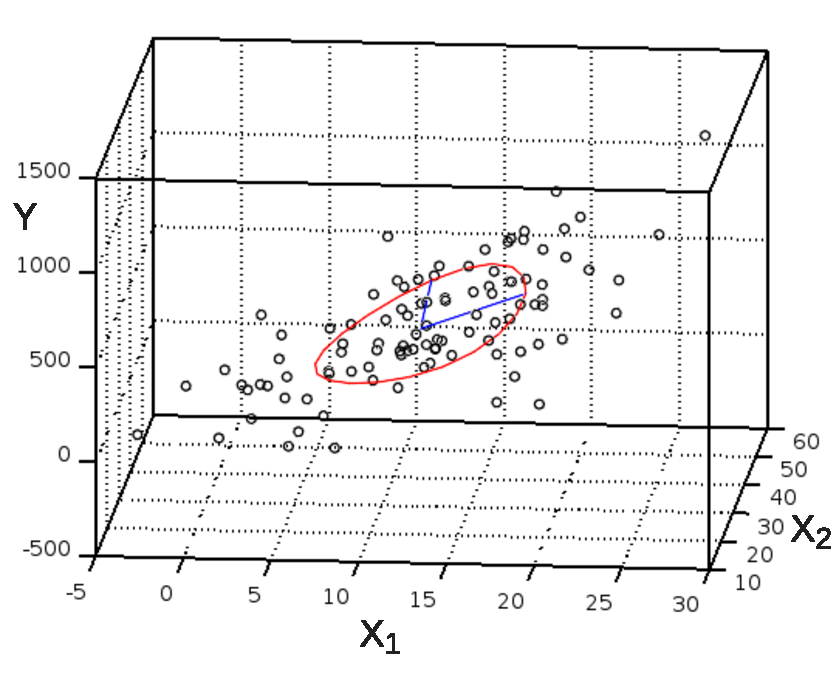
\includegraphics[width=100mm]{10_vorlesung_GUM/media/understand_fehlerfort_1.pdf}
\caption{\label{FortpfElliptisch} Eine anschauliche Deutung für die pythagoräische
Addition der Standardabweichungen liefert die Betrachtung der mit roter Kurve dargestellten
Ellipse. Die blauen Geraden repräsentieren die Abstände vom Mittelpunkt als Halbmesser
der Ellipse, die aus den Standardabweichungen jeweils von $X_1$ und $X_2$ berechnet wurden.}
\end{center}
\end{figure}
Da die beiden Größen $X_1$ und $X_2$ zwei unabhängige Dimensionen repräsentieren, werden
ihre Standardabweichungen nach dem Satz des Pythagoras addiert, eine Veranschaulichung dieses
Sachverhalts zeigt Abb.~\ref{FortpfElliptisch}. Da die Größen über die Modellgleichung
miteinander verknüpft sind und die gesuchte Standardabweichung die Dimension der Größe $Y$
trägt, müssen die Standardabweichungen der Größen $X_1$ und $X_2$ mit den entsprechenden
Sensitivitäten verknüpft werden, so dass
\begin{equation}
s_y^2 \; = \; (c_1 \, s_1)^2 \; + \; (c_2 \, s_2)^2 .
\end{equation}
Diese Varianz $s_y^2$ ist also wieder eine \textsl{kombinierte Varianz} und deren Wurzel
$s_y$ eine \textsl{kombinierte Standardabweichung}.

Für den allgemeinen Fall mit einer Linearsierung durch die Taylorreihenentwicklung
Gl.~(\ref{univarTaylorLin}) stellen die partiellen Ableitungen an
der Stelle der Schätzer der direkten Größen die Sensitivitäten
$c_i = \left. \frac{\partial f}{\partial X_i} \right|_{\bar{\mathbf{x}}}$ dar. Der
Vektor der partiellen Ableitungen heißt \textsl{Gradient}. Der Gradient ist also
der Steigungsvektor.
Der Gradient drückt aus, wie stark sich die indirekte Größe $Y$ gemäß der Steigung
des Kurvenverlaufs des Modells
ändert, wenn es kleine Änderungen der direkten Größen gibt. Mit anderen Worten besagt dies, wie
empfindlich die indirekte Größe auf Änderungen der direkten Größen reagiert, d.h.\ wie sensistiv
das Modell an der Position $\bar{\mathbf{x}}$ ist.

Gegeben sei ein univariates, expliziten Modell $Y = f(\mathrm{X})$, das linearisierbar ist, also
in Taylorreihe entwickelbar bis zum linearen Term mit dem Erwartungswertevektor
$\bar{\mathbf{x}}$ als Entwicklungspunkt
\begin{equation}
Y = f(\mathbf{X}) \approx \left. f(\mathbf{X}) \right|_{\bar{\mathbf{x}}} +
\sum_{i=1}^N \left.
\frac{\partial f}{\partial X_i} \right|_{\bar{\mathbf{x}}} \Delta X_i
\quad \text{und} \quad \mathrm{X} = \bar{\mathbf{x}} + \Delta \mathrm{X} .
\label{linearisiertesModellY}
\end{equation}
Die direkten Messgrößen $X_i$ sind Zufallsgrößen.
Bei der Linearisierung nehmen die Abweichungen $\Delta X_i$ der direkten Größen von ihren Erwartungswerten
$\mathrm{E}(X_i) = \bar x_i$ oder als Vektor mit den Erwartungswerten aller direkten Größen
$\bar{\mathbf{x}}$ die Rolle der Zufallsgrößen ein. Ihr Erwartungswert ist dann
Null $\mathrm{E}(\Delta X_i) = 0$.

Der Erwartungswert der indirekten Messgröße $Y$ wird durch Einsetzen der Erwartungswerte der
direkten Messgrößen in die Modellgleichung $Y = f(\mathrm{X})$ gewonnen
\begin{equation}
\mathrm{E}(Y) = \left. f(\mathbf{X}) \right|_{\bar{\mathbf{x}}}
\end{equation}

Zu der indirekten Messgröße soll die Varianz ermittelt werden
\begin{equation}
\operatorname{Var}(Y) =
\int \left(Y - E(Y) \right)^2 p(Y) \mathrm{d}Y =
\int \left(Y^2 - 2 Y \mathrm{E}(Y) + \mathrm{E}(Y)^2\right)  p(Y) \mathrm{d}Y
\end{equation}
mit $\int Y \mathrm{E}(Y) p(Y) \mathrm{d}Y = E(Y) \int Y p(Y) \mathrm{d}Y =
\mathrm{E}(Y) \mathrm{E}(Y)$ wird dies zu
\begin{equation*}
\operatorname{Var}(Y)
= \int \left(Y^2 - \mathrm{E}(Y)^2\right)  p(Y) \mathrm{d}Y
= \left(\int Y^2 p(Y) \mathrm{d}Y \right) - \mathrm{E}(Y)^2,
\end{equation*}
so dass gilt
\begin{equation}
\operatorname{Var}(Y)
= \int \left(Y^2 - \mathrm{E}(Y)^2\right)  p(Y) \mathrm{d}Y
= \int Y^2 p(Y) \mathrm{d}Y - \int \mathrm{E}(Y)^2  p(Y) \mathrm{d}Y .
\end{equation}
Hier wird der Ansatz Gl.~(\ref{linearisiertesModellY}) eingesetzt und mit
$p(Y)$ aus $p(X_1,\dots,X_N) = p(\mathbf{X})$ und mit
$\mathrm{d} \mathbf{X} = \mathrm{d} X_1\dots \mathrm{d} X_N$,
sowie mit $\int \mathrm{E}(Y)^2  p(Y) \mathrm{d}Y = \mathrm{E}(Y)^2$
\begin{equation}
\operatorname{Var}(Y)
= \int \left( \left. f(\mathbf{X}) \right|_{\bar{\mathbf{x}}} +
\sum_{i=1}^N \left.
\frac{\partial f}{\partial X_i} \right|_{\bar{\mathbf{x}}} \Delta X_i
 \right)^2
p(\mathbf{X}) \mathrm{d} \mathbf{X}
 \; - \; \mathrm{E}(Y)^2
\end{equation}
%\begin{small}
\begin{equation*}
= \int \left[ \left. f(\mathbf{X}) \right|_{\bar{\mathbf{x}}}^2 +
2   \left. f(\mathbf{X}) \right|_{\bar{\mathbf{x}}}
\sum_{i=1}^N \left.
\frac{\partial f}{\partial X_i} \right|_{\bar{\mathbf{x}}} \Delta X_i
+ \left(
\sum_{i=1}^N \left.
\frac{\partial f}{\partial X_i} \right|_{\bar{\mathbf{x}}} \Delta X_i
 \right)^2 \right]  p(\mathbf{X}) \mathrm{d} \mathbf{X}
\; - \mathrm{E}(Y)^2
\end{equation*}
%\end{small}
\begin{equation*}
= \int \left[
2   \left. f(\mathbf{X}) \right|_{\bar{\mathbf{x}}}
\sum_{i=1}^N \left.
\frac{\partial f}{\partial X_i} \right|_{\bar{\mathbf{x}}} \Delta X_i
+ \left(
\sum_{i=1}^N \left.
\frac{\partial f}{\partial X_i} \right|_{\bar{\mathbf{x}}} \Delta X_i
 \right)^2
\right]  p(\mathbf{X}) \mathrm{d} \mathbf{X}
\end{equation*}

\begin{equation*}
\operatorname{Var}(Y)
= \int \left[
2   \left. f(\mathbf{X}) \right|_{\bar{\mathbf{x}}}
\sum_{i=1}^N \left.
\frac{\partial f}{\partial X_i} \right|_{\bar{\mathbf{x}}} \Delta X_i
+ \left(
\sum_{i=1}^N \left.
\frac{\partial f}{\partial X_i} \right|_{\bar{\mathbf{x}}} \Delta X_i
 \right)^2
\right]  p(\mathbf{X}) \mathrm{d} \mathbf{X}
\end{equation*}
\begin{equation*}
= 2 \int   \left. f(\mathbf{X}) \right|_{\bar{\mathbf{x}}}
\sum_{i=1}^N \left.
\frac{\partial f}{\partial X_i} \right|_{\bar{\mathbf{x}}} \Delta X_i
\,  p(\mathbf{X}) \mathrm{d} \mathbf{X}
+ \int \left(
\sum_{i=1}^N \left.
\frac{\partial f}{\partial X_i} \right|_{\bar{\mathbf{x}}} \Delta X_i
 \right)^2
 p(\mathbf{X}) \mathrm{d} \mathbf{X}
\end{equation*}
\begin{equation*}
= 2 \left. f(\mathbf{X}) \right|_{\bar{\mathbf{x}}}  \sum_{i=1}^N \left.
\frac{\partial f}{\partial X_i} \right|_{\bar{\mathbf{x}}}
\underbrace{\int  \Delta X_i \, p(\mathbf{X}) \mathrm{d} \mathbf{X}}_{= 0}
+ \int \left(
\sum_{i=1}^N \left.
\frac{\partial f}{\partial X_i} \right|_{\bar{\mathbf{x}}} \Delta X_i
 \right)^2
 p(\mathbf{X}) \mathrm{d} \mathbf{X}
\end{equation*}

\begin{equation}
\operatorname{Var}(Y)
=
\int \left(
\sum_{i=1}^N \; \underbrace{
\left. \frac{\partial f}{\partial X_i} \right|_{\bar{\mathbf{x}}}}_{c_i} \;
\underbrace{\Delta X_i}_{X_i - E(X_i)}
 \right)^2
 p(\mathbf{X}) \mathrm{d} \mathbf{X}
=
\operatorname{Var}\left(\sum_{i=1}^N\underbrace{
\left. \frac{\partial f}{\partial X_i} \right|_{\bar{\mathbf{x}}}}_{c_i}  X_i\right)
\end{equation}

Als nächstes wollen wir wieder das Fortpflanzungsgesetz für die Messunsicherheit
in der Gestalt von Gl.~(\ref{univarLinearFortpflanzungKap7}) erhalten, wobei jetzt die Koeffizienten
$c_i$ die Steigungen der Tangenten $\frac{\partial f}{\partial X_i}$ an der Stelle
der geschätzten Erwartungswerte sind, d.h.\
$c_i = \left. \frac{\partial f}{\partial X_i} \right|_{\bar{\mathbf{x}}}$

\begin{equation}
\operatorname{Var}(Y)
= \operatorname{Var}\left(\sum_{i=1}^N c_i X_i\right)
\end{equation}
\begin{equation}
\operatorname {Var}\left(Y\right)
= \sum _{{i=1}}^{N} \, c_i^2 \operatorname {Var}( X_{i})+2\sum _{{i=1}}^{{N-1}}
  \sum _{{k=i+1}}^{N} \, c_i c_k \operatorname {Cov}(X_{i}, X_{k})
\label{UnsicherFortpflLinearisiert}
\end{equation}

Zu Kapitel 5.2 im JCGM 100-Dokument des \textsl{Guide} für Messunsicherheit GUM
sei angemerkt, dass für die Sensitivitäten eine verkürzte, unmathematische Schreibweise
für die Sensitivitäten gewählt wurde, indem dort geschrieben steht $\frac{\partial f}{\partial x_i}$
anstelle von $\left. \frac{\partial f}{\partial X_i} \right|_{\bar{\mathbf{x}}}$ oder
$\left. \frac{\partial f}{\partial X_i} \right|_{\bar x_1, \dots, \bar x_N}$.
Im GUM wird angemerkt, dass die saloppe Notation $\frac{\partial f}{\partial x_i}$ für
$\frac{\partial f}{\partial X_i}$
unter Verwendung der Schätzwerte $x_i$ zu den $X_i$ gewählt wird.
In unserer Vorlesungsreihe sowie im GUM steht das Symbol mit dem großgeschriebenen $X_i$ für die
direkten Messgrößen. Das im GUM verwendete $x_i$ als Kleinbuchstabe steht für den Schätzwert,
was wir in der Vorlesung mit $\bar x_i$ bezeichnen. Da der Schätzwert eine Konstante ist,
kann man nach dieser natürlich nicht ableiten.


\section{Überdeckungsintervall für indirekte Messgrößen}

Am Ende von Kapitel~\ref{konzepteStatistik} haben wir das Überdeckungsintervall eingeführt
und nach Einführung der Quantile der t-Verteilung in Kapitel~\ref{wahrscheinlichHyp} genauer
behandelt, als \textsl{Vertrauensintervall}, sowie im Zusammenhang der bayesischen Statistik
gewonnen aus der inversen kumulierten Posteriorverteilung als \textsl{Credible intervall}.

Die Intervallgrenzen des Vertrauensintervalls haben wir
auch als Produkt aus einem Quantil und einer Standardabweichung repräsentiert, im Fall, dass
eine Normalverteilung zugrunde gelegt wird in der Form
\begin{equation}
\left[\bar x \, - \, z_{1-\frac{1}{2}\alpha} \, \sigma_X,
\bar x \, + \, z_{1-\frac{1}{2}\alpha} \, \sigma_X \right]
\end{equation}
und im Fall, dass eine $t$-Verteilung zugrunde gelegt wird
\begin{equation}
\left[\bar x \, - \, t_{1-\frac{1}{2}\alpha, \nu} \, \sigma_X,
\bar x \, + \, t_{1-\frac{1}{2}\alpha, \nu} \, \sigma_X \right] .
\end{equation}
Bei dem Fall, dass eine $t$-Verteilung zugrunde gelegt wird, und zwar, wenn es um kleinere
Stichprobenumfänge geht, hängt das Quantil von der Anzahl der Freiheitsgrade $\nu_i = J_i - 1$
ab, die jedoch im allgemeinen für die beiden Größen $X_i$
unterschiedlich sein kann. Es gilt also, ein gemeinsames Quantil zu finden.

Mit der bayesischen Methode, die wir zuvor betrachtet haben, konnten wir das
\textsl{Credible Interval} aus der kumulierten Posterior gewinnen. Bei dem
zuvor erörterten Beispiel Gl.~(\ref{BeispielProdukt2Gr}) $Y = X_1 X_2$ haben wir statt
der einen Likelihood drei Verteilungsdichten:
Für jede Größe $X_i$ haben wir je eine Likelihood
\begin{equation}
p_{\mathrm{L},i}(\{X_{i,1}, \dots, X_{i,J}\} | X_i, s_i) \; = \;
\prod\limits_{j=1}^J \frac{1}{\sqrt{2 \pi} \, s_i}
 e^{- \frac{1}{2} \, \left( \frac{X_{i,j} - X_i}{s_i} \right)^2 }  \; = \;
l(X_i, s_i | \{X_{i,1}, \dots, X_{i,J}\})
\end{equation}
was zwei Verteilungen liefert, und als dritte Verteilung noch
\begin{equation}
p_\mathrm{L,y}( X_1, X_2 | Y, s) \; = \;
\frac{1}{\sqrt{2 \pi} \, s}
 e^{- \frac{1}{2} \, \left( \frac{Y - X_1 \, X_2}{s} \right)^2 }
\end{equation}
wobei dann nicht nur über $s$, sondern auch über $X_1$ und $X_2$ integriert wird, um die
Posterior als Marginalverteilung, die nur noch von $Y$ abhängt, zu erhalten.

Für relativ einfache analytische Zusammenhänge, also für explizite Modelle
und für ein\-fachere implizite Modellansätze wie die lineare Regression, ist
es nicht erforderlich die numerisch aufwendigere
kolmogoroff'sche Wahrscheinlichkeitsrechnung (Bildung
der Produkte der Verteilungen) anzuwenden.
Für explizite linearisierbare Modelle
$$
Y = f(\mathbf{X}) \qquad \mathbf{Y} = \vec f(\mathbf{X})
$$
mit $\vec f = (f_1,\dots,f_l, \dots, f_M)^\mathsf{T}$ ist das
Fortpflanzungsgesetz gemäß Gl.~(\ref{UnsichFortpfl2}) wie folgt
\begin{equation}
u^2(Y_l) = \sum\limits_{i=1}^{N} \, \left( \left. \frac{\partial f_l(\mathbf{X})}{\partial X_i}\right|_{\bar{\mathbf{x}}} \right)^2 \, u^2(X_i) \;  + \;
2 \, \sum\limits_{i=1}^{{N-1}}
 \sum\limits_{k=i+1}^{N} \, \left. \frac{\partial f_l(\mathbf{X})}{\partial X_i}\right|_{\bar{\mathbf{x}}} \,
 \left. \frac{\partial f_l(\mathbf{X})}{\partial X_k}\right|_{\bar{\mathbf{x}}}  \; \rho_{i,k} \, u(X_i) \, u(X_k)
\end{equation}
verwendbar. Für die lineare Regression
$$
Y_\mathrm{Regr} = \sum_{l=1}^M \theta_i X_l
$$
die bzgl.\ der indirekten Messgrößen $\theta_l = Y_l$ ein implizites Modell ist, gilt
für die Unsicherheitsfortpflanzung, die in Abschnitt~\ref{subsec:vertrauensbereiche}
dargelegt wird, siehe Gl.~(\ref{eq:Varianz des Achsenabschnitts}) bzw.\
Gl.~(\ref{eq:CovRegressparamsMatrix}) mit Gl.~(\ref{eq:URegressparamsMatrix}).
Mit einer Stichprobe mit Tupeln $(Y_{\mathrm{Regr},j}, X_{1,j},\dots,X_{M,j})$ und mit
$\boldsymbol Y_{\mathrm{Regr}} = (Y_{\mathrm{Regr},1},\dots,Y_{\mathrm{Regr},J})^{\mathsf{T}}$
und der Regressormatrix $\boldsymbol X = (X_{l,j})$ liefert das Fortpflanzungsgesetz die
Kovarianz der Modellparameter
\begin{equation}
\operatorname{Cov}(\boldsymbol \theta) \; = \; \left(\boldsymbol X^\mathsf{T} \, \boldsymbol X\right)^{-1} \, \operatorname{Var}(\boldsymbol \varepsilon)
\end{equation}
mit $J$ für den Stichprobenumfang und $M$ für die Anzahl der Modellparameter und mit
\begin{equation}
\operatorname{Var}(\boldsymbol \varepsilon) \; = \;
	\frac{1}{J-M}\left(\boldsymbol Y \; - \; \boldsymbol X \, \hat{\boldsymbol \theta}\right)^\mathsf{T}
\left(\boldsymbol Y \; - \; \boldsymbol X \, \hat{\boldsymbol \theta}\right) .
\end{equation}
Die Hauptdiagonale der Kovarianz der Modellparameter enthält die Varianzen
$$
\sigma_{\theta_l}^2 = u^2(\theta_l\equiv Y_l)
$$
der jeweiligen Modellparameter.

Für die Ermittlung des Überdeckungsintervalls $[y_l-U(Y_l), y_l+U_l]$ wird ein entsprechender
Erweiterungsfaktor $k$ für $U(Y_l) = k \, u(Y_l)$ gebraucht. Wird als Erweiterungsfaktor das
Quantil der $t$-Verteilung eingesetzt, so wird eine \textsl{effektive Anzahl
von Freiheitsgraden} $\nu_\mathrm{eff}$ approximiert.
In Abschnitt G.4 des Dokuments JCGM 100 GUM:2008 wird auf die Berechnungsmethode
für $\nu_\mathrm{eff}$ von Satterthwaite aus dem Jahr 1941 \cite{Sat41} zurückgegriffen.

Satterthwaite betrachtet die Varianz $\operatorname{Var}(s_i^2)$
der Varianz $s_i^2$. Die Varianzen $s_i^2$ sind unabhängige
Zufallsgrößen, also als Größen zu betrachten, die unkorreliert sind, so dass
\begin{equation}
\operatorname{Var}(s_y^2) \; = \;  \operatorname{Var}\left( c_1^2 s_1^2 \right)
 \; + \; \operatorname{Var}\left( c_2^2 s_2^2 \right)
\label{VarianzvarianzSumme}
\end{equation}
gilt.
Die empirischen Varianzen $s_1^2$ und $s_2^2$ der Größen $X_1$ und $X_2$ sind $\chi^2$-verteilt,
d.h.\ für die normierte Größe gilt
\begin{equation}
Q_i \; = \; \nu_i \, \left(\frac{s_i}{\sigma_i}\right)^2 \, \sim \; \chi^2(\nu_i) .
\end{equation}
Der Erwartungswert für $Q_i$ ist
\begin{equation}
\operatorname{E}(Q_i) \; = \; \int_0^\infty \; Q \; p_{\chi^2}(Q) \; \operatorname{d}Q \; = \; \nu_i.
\label{ErwartungswertQ}
\end{equation}
Die Varianz $\operatorname{Var}(Q_i)$ ist
\begin{equation}
\operatorname{Var}(Q_i) \; = \; \int_0^\infty \; (Q - \nu_i)^2 \; p_{\chi^2}(Q) \; \operatorname{d}Q \; = \; 2 \nu_i.
\label{VarianzQ}
\end{equation}
Die Herleitungen zu den beiden Gln.~(\ref{ErwartungswertQ}) und (\ref{VarianzQ})
befinden sich in Anhang \ref{ErwaChi2}.

Ferner gilt allgemein für die Varianz einer Zufallszahl $R$
multipliziert mit einem konstanten Faktor $a$
\begin{equation}
\arraycolsep=2.4pt\def\arraystretch{2}
\begin{array}{ll}
\operatorname{Var}(a R) & = \; \int\limits_0^\infty \, (a R - \operatorname{E}(a R))^2  \, p(R)  \, \operatorname{d}R \\
 & = \int\limits_0^\infty \, a^2 \, (R - \operatorname{E}(R))^2  \, p(R)  \, \operatorname{d}R\\
 & = a^2 \, \int\limits_0^\infty \, (R - \operatorname{E}(R))^2  \, p(R)  \, \operatorname{d}R\\
 & = a^2 \, \operatorname{Var}(R)
\end{array}
\end{equation}
so dass
\begin{equation}
\operatorname{Var}(Q_i) \; = \; \operatorname{Var}\left(\nu_i \, \left(\frac{s_i}{\sigma_i}\right)^2\right)
 \; = \; \left(\frac{\nu_i}{\sigma_i^2}\right)^2 \, \operatorname{Var}(s_i^2)
\end{equation}
mit Gl.~(\ref{VarianzQ}) wird dies zu
\begin{equation}
2 \nu_i \; = \; \left(\frac{\nu_i}{\sigma_i^2}\right)^2 \, \operatorname{Var}(s_i^2) .
\end{equation}
 Das heißt
\begin{equation}
2 \nu_i \; = \; \frac{\nu_i^2}{\sigma_i^4} \, \operatorname{Var}(s_i^2)
\end{equation}
%und
%\begin{equation}
%2 \sigma_i^4  \; = \; \frac{\nu_i^2}{\nu_i} \, \operatorname{Var}(s_i)
%\end{equation}
%und
%\begin{equation}
%2 \sigma_i^4  \; = \; \nu_i \, \operatorname{Var}(s_i)
%\end{equation}
also
\begin{equation}
\operatorname{Var}(s_i^2) \; = \; \frac{2 \sigma_i^4}{\nu_i} .
\end{equation}
so dass nach Sattherthwaite \cite{Sat41} aus Gl.~(\ref{VarianzvarianzSumme}) die \textsl{effektive Anzahl
der Freiheitsgrade} $\nu_\mathrm{eff}$ für die Größe $Y$, also $\nu_\mathrm{eff} = \nu_y$
abgeschätzt wird mit
$$
\frac{2 \sigma_y^4}{\nu_y} \; = \;  \frac{2 c_1^4 \sigma_1^4}{\nu_1}
 \; + \; \frac{2 c_2^4 \sigma_2^4}{\nu_2}
$$
mit $\operatorname{Var}(s_y^2) \; = \; \frac{2 \sigma_y^4}{\nu_y}$
und nach Rauskürzen des Faktors 2
\begin{equation}
\frac{\sigma_y^4}{\nu_y} \; = \;  \frac{c_1^4 \sigma_1^4}{\nu_1}
 \; + \; \frac{c_2^4 \sigma_2^4}{\nu_2}
\label{Satterthwaite}
\end{equation}
so dass
\begin{equation}
\nu_y \; = \; \frac{\sigma_y^4}{\frac{(c_1 \, \sigma_1)^4}{\nu_1}
 \; + \; \frac{(c_2 \, \sigma_2)^4}{\nu_2}} .
\label{EffectiveDFfuer2}
\end{equation}
Wenn mit Gleichung (\ref{ErwartungswertQ}) der Erwartungswert
von $Q$ gleich der Anzahl der Freiheitsgrade ist, also $\operatorname{E}(Q) = \nu$
für $Q = \nu \left(\frac{s}{\sigma}\right)^2$, dann ist der Erwartungswert der
Varianz $s^2$
\begin{equation}
\operatorname{E}(s^2) \; = \; \operatorname{E}(\frac{\sigma^2}{\nu} Q)
\end{equation}
und mit $\frac{\sigma^2}{\nu}$ als konstanter Faktor bezüglich der Wahrscheinlichkeitsdichte
und mit Gl.~(\ref{ErwartungswertQ}) erhalten wir
\begin{equation}
\operatorname{E}(s^2) \; = \; \frac{\sigma^2}{\nu}  \operatorname{E}(Q) \; = \;
\frac{\sigma^2}{\nu} \nu \; = \; \sigma^2
\end{equation}
und wir setzten in Gl.~(\ref{EffectiveDFfuer2}) die Erwartungswerte
$\operatorname{E}(s_y^2)$, $\operatorname{E}(s_1^2)$ und $\operatorname{E}(s_2^2)$ ein,
deren Schätzer die empirisch ermittelten Varianzen sind.

Das $t$-Quantil wird damit für $\nu_y = \nu_\mathrm{eff}$ berechnet und das vollständige Messergebnis wie folgt
angegeben
\begin{equation}
Y \; = \; y \, \pm \, t_{1-\alpha/2,\nu_y} s_y .
\label{vollstaendigesSatterthwaite}
\end{equation}


Verallgemeinert für $N$ direkte Größen ist dies
\begin{equation}
\nu_\mathrm{eff} \; = \; \frac{\sigma_y^4}{\sum\limits_{i=1}^N \frac{(c_i \, \sigma_i)^4}{\nu_i}} .
\label{EffectiveDFviele}
\end{equation}


Aufgrund der Verallgemeinerung, dass \textsl{Überdeckungsintervalle} sowohl
klassisch ermittelte Vertrauensintervalle als auch bayesisch ermittelte
\textsl{Credible Intervals} sein können,
werden die zu einer gewissen Wahrscheinlichkeit $1-\alpha$ gehörenden Faktoren
\textsl{Erweiterungsfaktor} genannt. Sei  $[z_\mathrm{min}, z_\mathrm{max}]$
das \textsl{Credible Interval}
einer Größe $Y$ mit Posterior $p(Y |\dots)$ deren Erwartungswert
\begin{equation}
\bar Y \; = \; \int\limits_{-\infty}^\infty \, Y \, p(Y |\dots) \, \operatorname{d}Y
\end{equation}
und deren Varianz
\begin{equation}
\operatorname{Var}(Y) \; = \; \int\limits_{-\infty}^\infty \, (Y - \bar Y)^2 \, p(Y |\dots) \, \operatorname{d}Y
\end{equation}
ist, so ist der \textsl{Erweiterungsfaktor} $k$ für symmetrische Verteilungen mit
$z_\mathrm{max} - \bar Y = \bar Y - z_\mathrm{min}$
\begin{equation}
k \; = \; \frac{z_\mathrm{max} - \bar Y}{\sqrt{\operatorname{Var}(Y)}}
\end{equation}
was für klassische Berechnungsverfahren dem
t-Quantil $t_{1-\alpha/2,\nu_\mathrm{eff}}$ entspricht
\begin{equation}
k \; = \; t_{1-\alpha/2,\nu_\mathrm{eff}} .
\end{equation}
Für symmetrische Verteilungen ist die halbe Breite des Überdeckungsintervalls
gleich der \textsl{erweiterten Messunsicherheit} der Größe $Y$. Die
\textsl{erweiterte Messunsicherheit} kann das Produkt aus
Erweiterungsfaktor und empirischer Standardabweichung sein.

Während mit \textsl{kleinem} Buchstaben $u$ die Standardabweichungen bezeichnet werden,
werden mit \textsl{großem} Buchstaben $U$ die erweiterten Unsicherheiten geschrieben. Die
erweiterten Unsicherheiten sind das Produkt aus
dem Erweiterungsfaktor $k$, der in der klassischen Statistik das $t$-Quantil ist,
und der Unsicherheit $u$.


\section{Aufgabe zum Selbststudium}
\label{AufgVor7}
Es sollen Abstände auf einem Werkstück mit Hilfe eines induktiven Wegaufnehmers gemessen werden.
Das Messprinzip eines induktiven Wegaufnehmers beruht darauf, dass
eine Wechselspannung ein Spulensystem im Sensor anregt.
Ein bewegliches ferro-magnetisches Teil am Sensor
beeinflusst die Induktivität in den Spulen.
Diese - in den Spulenteilen unterschiedliche - Induktivitätsveränderung wird vom
Messverstärker ausgewertet und in ein positions-proportionales Gleichspannungssignal
umgewandelt.

Um die Abstände in der physikalischen Einheit Mikrometer zu erhalten, muss mit Hilfe
eines Bezugsnormals aus dem Spannungssignal ein Weg mit der Dimension einer Länge
berechnet werden.
Es ist bekannt, dass in dem für die Messung relevanten Messbereich (Hub des Sensors)
die Abhängigkeit zwischen Spannungssignal und Auslenkung des ferro-magnetischen Kerns
linear ist.
Das Bezugsnormal ist eine Stufenhöhe.

Zu dem Bezugsnormal gibt es einen Kalibrierschein, der folgenden Höhenwert für das
Normal angibt:
\begin{equation}
d \; = \; (4.997 \pm 0.011) \; \mathrm{\mu m} \qquad \mathrm{mit} \qquad k = 2.1, \nu = 26
\label{kalBezug}
\end{equation}

Mit dem induktiven Wegaufnehmer wurden auf dem Bezugsnormal folgende Stufenhöhen in
der Dimension der elektrischen Spannung mit der Einheit Millivolt gemessen

% muB = 200; sigB = 8;
% JB = 11; xB = muB+sigB*randn(1,JB);
% printf("& %4.1f ", xB);
% xB = [201.3  187.3  196.5  200.4  193.6  174.2  197.2  185.4  194.4  202.5  205.2];
Tabelle A5.1:\\
\begin{tabular}{c||c|c|c|c|c|c|c|c|c|c|c}
\hline
$U_\mathrm{B} / \mathrm{mV}$ & 201.3 & 187.3 & 196.5 & 200.4 & 193.6 & 174.2 & 197.2 & 185.4 & 194.4 & 202.5 & 205.2\\
\hline
\end{tabular}

%Für den Abstand auf dem Werkstück wurden folgende Spannungen gemessen
%>> muW = 180; sigW = 11;
%>> JW = 7; xW = muW+sigW*randn(JW,1);
%>> printf(" %4.1f ", xW);
% 176.5  184.1  180.5  193.6  176.0  194.5  160.9 >>
%>> printf("& %4.1f ", xW);
Tabelle A5.2:\\
\begin{tabular}{c||c|c|c|c|c|c|c}
\hline
$U_\mathrm{W} / \mathrm{mV}$ & 176.5 & 184.1 & 180.5 & 193.6 & 176.0 & 194.5 & 160.9 \\
\hline
\end{tabular}

Der Zusammenhang zwischen dem Abstand auf dem Werkstück in Mikrometern $d_\mathrm{W}$,
der Stufenhöhe des Bezugsnormals gemäß Kalibrierschein $d$, dem gemessenen Spannungssignal
an der Stufenhöhe $U_\mathrm{B}$ und dem gemessenen Spannungssignal $U_\mathrm{W}$ am Werkstück
ist folgender
\begin{equation}
d_\mathrm{W} \; = \; \frac{d}{U_\mathrm{B}} \, U_\mathrm{W}
\end{equation}

Die Änderungen aufgrund der statistischen Streuung der Spannungswerte $U_\mathrm{B}$ sind
so klein, dass für die Sensitivität $c_\mathrm{B}$ von $d_\mathrm{W}$
bezüglich Änderungen von $U_\mathrm{B}$
mit dem hyperbolischen Zusammenhang $d_\mathrm{W} \sim \frac{1}{U_\mathrm{B}}$
die Steigung der Tangenten an die Hyperbel verwendet wird. Es wird die
Tangente verwendet, die an dem Punkt, der sich aus den Mittelwerten
ergibt, anliegt.
\begin{equation}
c_\mathrm{B} \; = \; \left. \frac{\partial}{\partial U_\mathrm{B}}
 d_\mathrm{W} \right|_{\bar U_\mathrm{B}, \bar d, \bar U_\mathrm{W}}
\end{equation}
Die Sensitivitäten $c_\mathrm{d}$ und $c_\mathrm{W}$ von $d_\mathrm{W}$
bezüglich Änderungen von $d$ und $U_\mathrm{W}$ sind aufgrund des
linearen Zusammenhangs genau
\begin{equation}
c_\mathrm{d} \; = \; \left. \frac{U_\mathrm{W}}{ U_\mathrm{B}} \right|_{\bar U_\mathrm{B}, \bar U_\mathrm{W}} \qquad
c_\mathrm{W} \; = \; \left. \frac{d}{U_\mathrm{B}} \right|_{\bar U_\mathrm{B}, \bar d}
\end{equation}
definiert.
Die kombinierte Varianz unter der Voraussetzung, dass die gemessenen Größen und
die Angabe aus dem Kalbrierschein unkorreliert sind, ist
\begin{equation}
s_\mathrm{dW}^2 \; = \; (c_\mathrm{d} \, s_\mathrm{d})^2 \; + \;
(c_\mathrm{B} \, s_\mathrm{B})^2 \; + \; (c_\mathrm{W} \, s_\mathrm{W})^2
\end{equation}
mit $s_\mathrm{B}$ für die Standardabweichung der in Tabelle A5.1 aufgelisteten Werte,
$s_\mathrm{W}$ für die Standardabweichung der in Tabelle A5.2 aufgelisteten Werte und
$s_\mathrm{d}$ für die Standardabweichung der Angabe aus dem Kalibrierschein.

\begin{itemize}
\item[a)] Ermitteln Sie aus den Angaben des Kalibrierscheins (hier Gl.~(\ref{kalBezug}))
die Standardabweichung $s_\mathrm{d}$, indem Sie den dort genannten Erweiterungsfaktor verwenden.
%>> d = 4.997 d =  4.9970
%>> sd = 0.011/2.1 sd =  0.0052381
\item[b)] Ermitteln Sie die beiden Mittelwerte $\bar U_\mathrm{B}$ und $\bar U_\mathrm{W}$,
sowie die beiden empirirschen Standardabweichungen $s_\mathrm{B}$ und $s_\mathrm{W}$
aus den beiden Tabellen A5.1 und A5.2.
%>> xBbar = mean(xB) xBbar =  194.36
%>> xWbar = mean(xW) xWbar =  180.85
%>> sW = std(xW) sW =  11.561
%>> sW2 = var(xW) sW2 =  133.65
%>> sB = std(xB) sB =  9.0410
%>> sB2 = var(xB) sB2 =  81.739
\item[c)] Bestimmen  Sie die Sensitivitäten $c_\mathrm{d}$, $c_\mathrm{W}$, $c_\mathrm{B}$ durch Ausführen der
partiellen Ableitung.
%(%i4) dW(UB) := UW*d/UB;
%                                          UW d
%(%o4)                           dW(UB) := ----
%                                           UB
%(%i5) diff(dW(UB),UB);
%                                      d UW
%(%o5)                               - ----
%                                        2
%                                      UB
\item[d)] Berechnen Sie die kombinierte empirische Standardabweichung $s_\mathrm{dW}$.
%>> cd = xWbar/xBbar cd =  0.93048
%>> cW = d/xBbar cW =  0.025710
%>> cB = -d*xWbar/(xBbar^2) cB = -0.023922
%s2 = (sd*cd)^2 + sW2*cW^2 + sB2*cB^2 s2 =  0.13514
%s = sqrt((sd*cd)^2 + sW2*cW^2 + sB2*cB^2) s =  0.36762
\item[e)] Berechnen Sie die effektive Anzahl der Freiheitsgrade.
%nueff = s2^2 / ((sd*cd)^4/26 + (sW2*cW^2)^2/(JW-1) + (sB2*cB^2)^2/(JB-1)) nueff =  12.019
\item[f)] Berechnen Sie den Erweiterungsfaktor $k$, der
 hier das t-Quantil für ein zweiseitiges Vertrauensniveau
 von $1-\alpha = 0.95\%$ ist.
% k=tinv(0.975,nueff) k =  2.1784
\item[g)] Bestimmen Sie das vollständige Messergebnis.
% dW = d*xWbar/xBbar  dW =  4.6496
% k*s =  0.80083
% d_W = 4.6496 \pm 0.80083
\end{itemize}
